\documentclass[12pt]{article}
\textwidth=17cm \oddsidemargin=-0.9cm \evensidemargin=-0.9cm
\textheight=23.7cm \topmargin=-1.7cm

\usepackage{amssymb, amsmath, amsfonts}
\usepackage{moreverb}
\usepackage{graphicx}
\usepackage{enumerate}
\usepackage{graphics}
\usepackage{color}
\usepackage{array}
\usepackage{float}
\usepackage{hyperref}
\usepackage{textcomp}
\usepackage{alltt}
\usepackage{physics}
\usepackage{mathtools}
\usepackage{tikz}
\usetikzlibrary{positioning}
\usetikzlibrary{arrows}
\usepackage{pgfplots}
\usepackage{bigints}
\usepackage[utf8]{inputenc}
\usepackage[english]{babel}
\usepackage{amsthm}
\usepackage{fancyhdr}
\usepackage[makeroom]{cancel}
\usepackage{cite}
\usepackage{subcaption}
\pagestyle{fancy}
\allowdisplaybreaks

\newcommand{\E}{\varepsilon}

\newcommand{\suchthat}{\, \mid \,}
\newcommand{\ol}[1]{\overline{#1}}
\newcommand{\bbar}[1]{\overline{#1}}
\newcommand{\inpd}[1]{{\left< \, #1 \, \right>}}
\renewcommand{\theenumi}{\alph{enumi}}
\newcommand\Wider[2][3em]{%
\makebox[\linewidth][c]{%
  \begin{minipage}{\dimexpr\textwidth+#1\relax}
  \raggedright#2
  \end{minipage}%
  }%
}

\def\R{\mathbb{R}}
\def\C{\mathbb{C}}
\def\H{\mathcal{H}}
\DeclareMathOperator*{\esssup}{\text{ess~sup}}
\newcommand{\resolv}[1]{\rho(#1)}
\newcommand{\spec}[1]{\sigma(#1)}
\newcommand{\iffR}{\noindent \underline{$\Longrightarrow$:} }
\newcommand{\iffL}{\noindent \underline{$\Longleftarrow$:} }
\newcommand{\lightning}{\textbf{\Huge \Lightning}}
\newcommand{\spt}[1]{\text{spt}(#1)}
\def\ran{\text{ ran}}
   
\setcounter{section}{0}

%%%% BIGGER FIGURES, tex studio?


\begin{document}
\lhead{Carter Johnson}
\chead{ECL 233 Term Project Idea}
\rhead{\today}


I'm working on a paper with Prof. Hastings on the effect of migration on resilience in the two-population differential equation model
\begin{align}
\dot{X_1} = X_1 (K_1 - (X_1 - 1)^2) + D( X_2 - X_1) \label{equation_2} \\
\dot{X_2} = X_2 (K_2 - (X_2 - 1)^2) + D( X_1 - X_2). \label{equation_3}
\end{align}


Each population exhibits either a Strong Allee effect, Weak Allee effect, or fatal Allee effect according to some parameter K, leading to a saddle-node bifurcation in K.

\begin{equation}\label{equation_1}
\dot{X} = X ( K - (X-1)^2).
\end{equation}


\begin{figure}[H]\label{bifd_1d}
\centering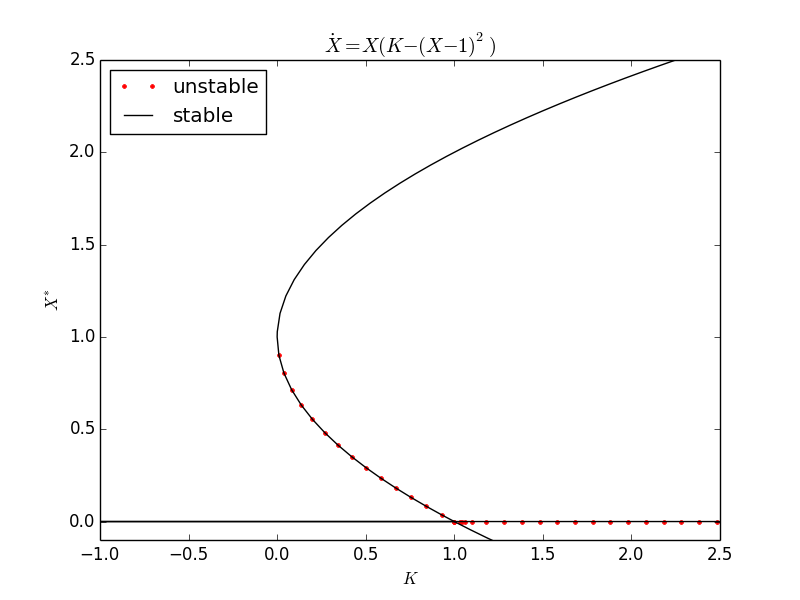
\includegraphics[scale=0.65]{single_pop_bif_diag_ver3.png}
\caption{The bifurcation diagram for equation (\ref{equation_1}) with bifurcation parameter $K$.  Note the three regimes: $K<0
$ Fatal Allee Effect/ Extinction; $0 < K < 1$ Strong Allee Effect / Bistability; $K > 1$ Weak Allee Effect.}
\end{figure}

The effects on resilience can be summarized by the following bifurcation diagrams:

\begin{figure}[H]
\centering
\begin{subfigure}{.5\textwidth}
  \centering
	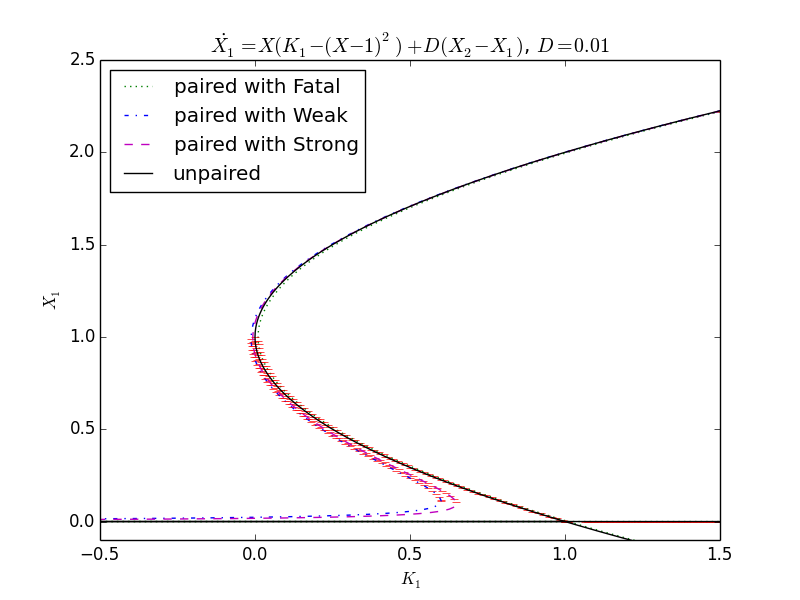
\includegraphics[scale=0.4]{shifted_bifds_001D.png}
	\end{subfigure}%
\begin{subfigure}{.5\textwidth}
  \centering
	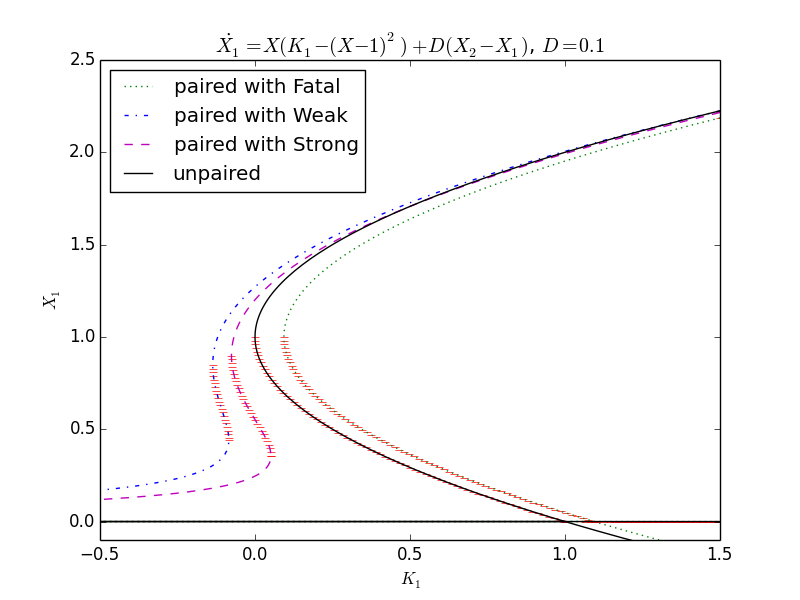
\includegraphics[scale=0.4]{shifted_bifds_01D.png}
\end{subfigure}
\caption{(a) shows $D=0.01$; note the loss of the transcritical bifurcation for $X_1$ for the pairings to Strong and Weak regimes of $X_2$. (b) shows $D=0.1$; note the leftward shift of the saddle-node bifurcation for the pairings to Strong and Weak regimes. For the coupling to the Strong and Weak paired regimes, $X_2$ was at its high-level stable state, and for the coupling to the Fatal paired regime, $X_2$ was at its low-level stable state.}
\label{comparing_bifds} 
\end{figure}


The next step in my analysis is to add stochasticity to the differential equations and see how the resilience plays out.  My idea for this project would be to come up with a few plots showing the effects of stochasticity in this system, which I hope to learn how to do by the end of this course. 

\end{document}